\section{Low-rank subspace clustering with prior knowledge}
\label{sec:lowrank}
In this section, we present our low-rank subspace clustering framework with prior knowledge, based on which our normal estimation algorithm is designed (Section \ref{sec:algorithm}). First, we give a short review of subspace clustering. Subspace clustering is a fundamental problem which has numerous
applications in image processing and computer vision.
%
In practice, the data points are always drawn from a union of subspaces with lower intrinsic dimensions than the dimension of the ambient space.
The task of subspace clustering is to segment the data into multiple
low-dimensional linear subspaces.

\subsection{Sparse subspace clustering (SSC)}
\label{sec:subspacesegmentation}
The recently proposed sparse representation, low-rank representation achieves competitive results in subspace clustering~\cite{DBLP:journals/corr/abs-1010-2955,LiuLY10,DBLP:conf/cvpr/ElhamifarV09}. These methods are all based on the observation that a data vector can be represented by
the data vectors from the same subspace and their models can be summarized as follows
\begin{eqnarray}
min f(Z) & s.t. & X=XZ,
\end{eqnarray}
where $f(Z)$ is a matrix function, each column of the matrix $X$
represents a sample. The affinity matrix $S$ can be defined as
\begin{eqnarray}
S=|Z|+|Z'|. \label{eq:defineS}
\end{eqnarray}
Then the NCut method \cite{DBLP:journals/pami/ShiM00} is applied to get the
clustering result. The key of these methods is to
define an appropriate function $f$.


Sparse subspace clustering (SSC) proposed by E. Elhamifar \etal
~\cite{DBLP:conf/cvpr/ElhamifarV09} uses the 1D sparsity. It is an
effective method for the independent subspace clustering and the
model can be written as
\begin{eqnarray}
min \|Z\|_{1} & s.t. & X=XZ,diag(Z)=\textbf{0},
\end{eqnarray}
where $\|\cdot\|_{1}$ represents $l_{1}$-norm. However,
\cite{DBLP:conf/cvpr/NasihatkonH11} gives failure examples in dimensions higher than three. Moreover, SSC finds the sparsest
representation of each sample individually without global
constraints.
\subsection{Low-rank subspace clustring (LRSC)}
\label{sec:LRSC}
To capture the global structure of
the whole data, low-rank representation~\cite{DBLP:journals/corr/abs-1010-2955,LiuLY10}
considering the 2D sparsity, \ie the rank of a matrix, is presented for subspace clustering.
The model can be written as
\begin{eqnarray}
min \|Z\|_{*} & s.t. & X=XZ,
\end{eqnarray}
where $\|\cdot\|_{*}$ represents the sum of singular value. It is an effective subspace clustering algorithm that outperforms the state-of-the-art algorithms in handling corrupted data. However, when the subspaces are not independent, this method may fail.

%\jj{Zhuang can for dependent?} Thus Zhuang \etal
%~\cite{DBLP:conf/cvpr/ZhuangGLMZY12} proposed Non-Negative Low-Rank and Sparse (NNLRS) graph for semi-supervised learning, which can be written as
%\begin{eqnarray}
%min \|Z\|_{*} + \beta\|Z\|_{1} & s.t. & X=XZ,Z\geq \textbf{0},
%\label{eq:NNLRS}
%\end{eqnarray}
%where $\beta \geq 0$ is used to balance the influence of these two terms. This method considers both the sparsity and the global structure by combining 1D sparsity with 2D sparsity.

\subsection{Low-rank subspace clustering with prior knowledge (LRSCPK)}
\label{sec:LRSCPK}
To segment two or more intersection planes, an affinity matrix which is
dense between same class and sparse between different classes is preferred.
%
Thus we propose a low-rank subspace clustering framework (LRSCPK) with prior knowledge:
\begin{eqnarray}
min \|Z\|_{*} + \beta\|\mathcal {P}_{\Omega}(Z)\|_{1} & s.t. &
X=XZ.\label{eq:SSLRR}
\end{eqnarray}
where $\Omega$ is a guiding matrix and $0 \leq \Omega(i,j) \leq 1$,
$\mathcal {P}_{\Omega}$ can be seen as a mapping satisfying $\mathcal {P}_{\Omega}(Z)_{i,j} = \Omega(i,j)\times Z(i,j)$.
The guiding matrix $\Omega$ can be seen as prior knowledge. $\Omega$ has the property that the samples from the same
intra class contribute to a smaller weight while the samples from interclass contribute to a larger weight.
We note that the subspace can be clustered correctly even when $\Omega$ contains partial prior and gentle noise in our experiments.

%
In order to improve the robustness of this method, we replace the equality constraint of problem (\ref{eq:SSLRR}) with a soft constraint
\begin{small}
\begin{eqnarray}
min \|Z\|_{*} + \beta\|\mathcal {P}_{\Omega}(Z)\|_{1} +
\gamma\|E\|_{2,1} & s.t. & X=XZ+E, \label{eq:RSSLRR}
\end{eqnarray}
\end{small}
where $\beta$ and $\gamma$ are two parameters and we set them as 1 in this work, $\|\cdot\|_{2,1}$ is the $l_{2,1}$ norm and defined as the sum of $l_{2}$ norms of the columns of a matrix.
%To verify the effectiveness and robustness of the framework, a toy example is provided.

\subsubsection{A toy example}
\label{sec:toy}
A toy example is provided to verify the effectiveness and robustness of LRSCPK.
We sample $300$ points from two intersecting planes in $\mathbb{R}^{3}$, $150$ for
each plane.
%
Forty percent prior knowledge with $20\%$, $30\%$, $40\%$ errors are presented to LRSCPK.
%
Specifically, the ideal full guiding matrix $G\in \mathbb{R}^{300*300}$ has the property
that if two samples $p_{j}$ and $p_{k}$ are in the same plane, $G(j,k) = 0$,
otherwise $G(j,k) = 1$.
%
The guiding matrix $\Omega$ is generated by choosing $40\%$ elements of $G$ randomly and the other elements of $\Omega$ are all zeros. The errors are added by randomly selecting $20\%$, $30\%$, $40\%$ elements from the $40\%$ elements and switching their values, \ie from ones to zeros if they are ones originally (resp. zero to one).
%
As illustrated by~\fig~\ref{fig:improve} (a), (b) and (c), LRSC fails to segment two dependent subspaces, while LRSCPK generates faithful segmentation using partial prior knowledge even with considerable levels of errors.
Moreover, when the prior knowledge is seriously corrupted by errors, LRSCPK still provides a more qualified segmentation than LRSC, as shown in~\fig~\ref{fig:improve} (d).
\begin{figure*}[htbp]
\begin{center}
    \begin{tabular}{c}
        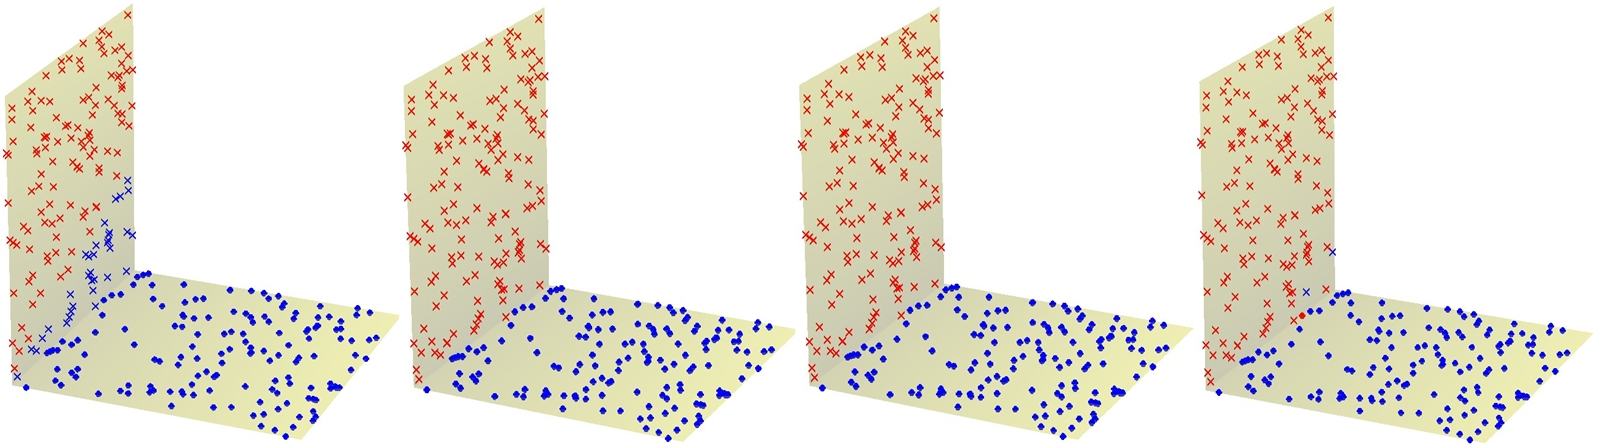
\includegraphics[width=1\linewidth]{test}\\
        \hspace{-10 mm} (a) \hspace{34 mm} (b) \hspace{34 mm} (c)\hspace{34 mm} (d)
    \end{tabular}
    \caption{Segmentation results of LRR and LRSCPK on two intersecting planes. (a) The result of LRR with $11\%$ clustering error. From (b) to (d) are the results of LRSCPK with $40\%$ prior knowledge which are corrupted by $20\%$, $30\%$ and $40\%$ errors, respectively. The clustering error is 0, 0 and $1\%$.}
    \label{fig:improve}
\end{center}
\end{figure*}
